\documentclass[a4paper, 10pt]{article}

\usepackage{../packages}

\graphicspath{{./figures}}



\begin{document}
\begin{titlepage}
\begin{center}
	
\includegraphics[scale=0.7]{logo.png}

	\vspace*{4cm}
	\textbf{Bazy danych\\ Laboratorium}

	\vspace{1.5cm}
	\textit{Zarządzanie bazą danych Oracle}

	\vspace{1.5cm}
	\textbf{Stanislau Antanovich}\\
	nr. indeksu: 173590\\
	gr. lab: L04

	\vspace{4.5cm}
	%\today
\end{center}
\end{titlepage}

\tableofcontents
\listoffigures
\lstlistoflistings

\newpage

\section{Realizacja}

\begin{enumerate}
	\item Tworzenie przestrzeni TABLESPACE o nazwie ``\emph{project\_tablespace}''.
		\begin{lstlisting}[style=SQL, caption=\textit{Tworzenie przestrzeni TABLESPACE o nazwie ``project\_tablespace''}]
CREATE TABLE SPACE project_tablespace
DATAFILE 'project_tablespace.dbf' SIZE 100M
AUTOEXTEND ON NEXT 10M MAXSIZE UNLIMITED;
		\end{lstlisting}
		\begin{figure}[H]
			\centering
			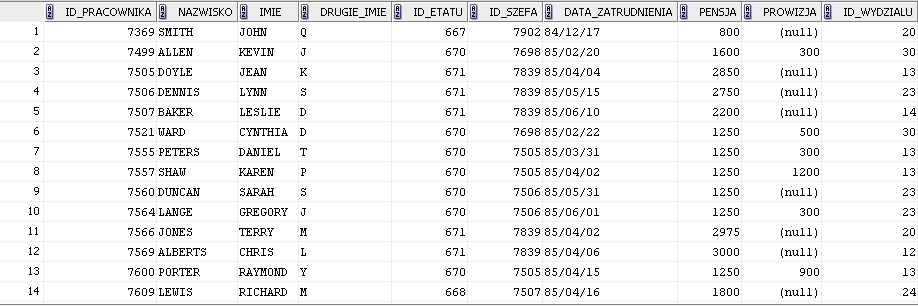
\includegraphics{zadanie1.png}
			\caption{\textit{Tworzenie przestrzeni TABLESPACE o nazwie ``project\_tablespace''}}
		\end{figure}
	\item Tworzenie używtkownika dla nowej bazy danych oraz przestrzeni o danych:
		\begin{itemize}
			\item nazwa: ``student1''
			\item hasło: zgodnym z dniem tworzenia np. ``07052023''
		\end{itemize}
		Przypisanie do konta użytwkownika przestrzeń ``\emph{project\_tablespace}'' oraz odpowiednie dostępy oraz role.
		\begin{lstlisting}[style=SQL, caption=\textit{Tworzenie użytkownika}]
CREATE USER student1 IDENTIFIED BY ``07052023'';
ALTER USER student1 DEFAULT TABLESPACE project_tablespace;
GRANT ALL PRIVILEGES TO student1;
		\end{lstlisting}
	\item Wdrożenie bazy danych. 
		\begin{lstlisting}[style=SQL, caption=\textit{Wdrożenie bazy danych}]
CREATE TABLE student (
	id INTEGER PRIMARY KEY,
	name VARCHAR2(255),
	surname VARCHAR2(255),
	index_num INTEGER
);

CREATE TABLE topic(
	id INTEGER PRIMARY KEY,
	name VARCHAR2(255)
);

CREATE TABLE assignment(
	student_id INTEGER,
	topic_id INTEGER,
	start_date DATE,
	rating FLOAT,
	FOREIGN KEY (student_id) REFERENCES student(id),
	FOREIGN KEY (topic_id) REFERENCES topic(id)
);

CREATE TABLE topic_assignment(
	topic_id INTEGER,
	assignment_id INTEGER
);

CREATE TABLE issue(
	id INTEGER PRIMARY KEY,
	name VARCHAR2(255),
	topic_id INTEGER,
	FOREIGN KEY (topic_id) REFERENCES topic(id)
);
		\end{lstlisting}
		\begin{figure}[H]
			\centering
			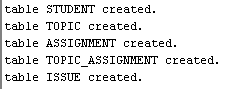
\includegraphics{zadanie3.png}
			\caption{\textit{Wdrożenie bazy danych}}
		\end{figure}
	\item Tworzenie sekwencji ``\emph{student\_seq}'' dedykowaną dla studenta w przedziale od 0 do 10000.
		\begin{lstlisting}[style=SQL, caption=\textit{Tworzenie sekwencji ``student\_seq''}]
CREATE SEQUENCE student_seq
START WITH 1
INCREMENT BY 1
MAXVALUE 10000
NOCYCLE
NOCACHE;
		\end{lstlisting}
		\begin{figure}[H]
			\centering
			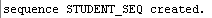
\includegraphics{zadanie4.png}
			\caption{\textit{Tworzenie sekwencji ``student\_seq''}}
		\end{figure}
	\item Funkcja, która pozwala dodać nowego studenta (addStudent). Wykorzystanie utworzonej sekwencji ``\emph{student\_seq}'' dla ustalenia kolejnego ID. Zwracanie z funkcji ID dodanego studenta.
		\begin{lstlisting}[style=SQL, caption=\textit{Funkcja, która dodaje nowego studenta}]
CREATE OR REPLACE FUNCTION addStudent(
	p_name IN VARCHAR2,
	p_surname IN VARCHAR2,
	p_index_num IN INTEGER
) RETURN INTEGER IS
v_id INTEGER;
BEGIN
	SELECT student_seq.NEXTVAL INTO v_id FROM DUAL;
	INSERT INTO student (id, name, surname, index_num)
	VALUES (v_id, p_name, p_surname, p_index_name);
	RETURN v_id;
END;
		\end{lstlisting}
		\begin{figure}[H]
			\centering
			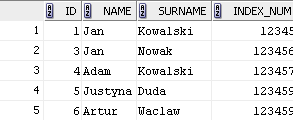
\includegraphics[scale=0.6]{zadanie5.png}
			\caption{\textit{Funkcja, która dodaje nowego studenta}}
		\end{figure}
	\item Wprowadzenie danych do tablicy. Wywołanie funkcji addStudent.
		\begin{figure}[H]
			\centering
			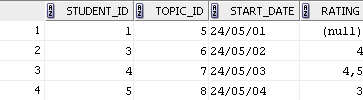
\includegraphics[scale=0.6]{zadanie6_1.png}
			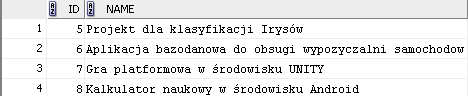
\includegraphics[scale=0.46]{zadanie6_2.png}\\
			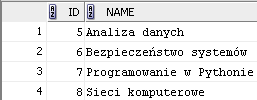
\includegraphics[scale=0.84]{zadanie6_3.png}
			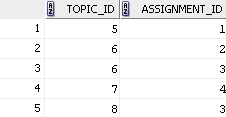
\includegraphics[scale=0.95]{zadanie6_4.png}
			\caption{\textit{Wprowadzenie danych do tablicy}}
		\end{figure}
	\item Tworzenie widoków odpowiedzialnych za:
		\begin{itemize}
			\item wyświetlenie wszystkich tematów projektów 
			\item wyświetlenie wszystkich studentów, którzy nie mają przypisanego tematu
		\end{itemize}
		\begin{lstlisting}[style=SQL, caption=\textit{Tworzenie widoków}]
CREATE OR REPLACE VIEW topcis AS
SELECT name
FROM topic;
CREATE OR REPLACE VIEW  students_lacking_topic AS
	SELECT * 
	FROM student WHERE NOT EXISTS (
	SELECT 1
	FROM assignment
	WHERE assignment.student_id=student.id
);
		\end{lstlisting}
		\begin{figure}[H]
			\centering
			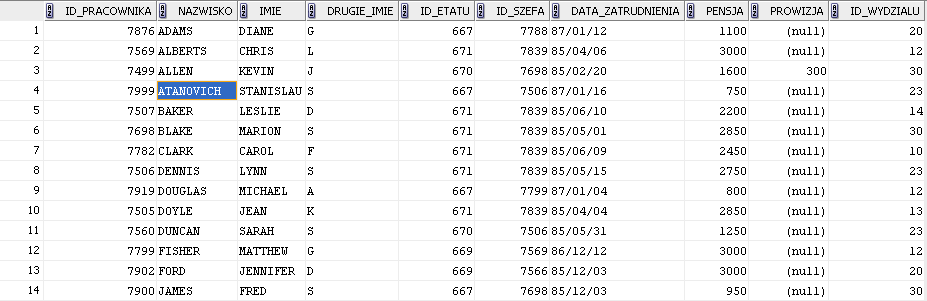
\includegraphics{zadanie7.png}
			\caption{\textit{Tworzenie widoków}}
		\end{figure}
	\item Zwracanie raportu do pliku o rozszerzeniu \emph{.csv} z informacją o nagłówku(kolumny):
		\begin{itemize}
			\item dane studenta(indeks, imię oraz nazwisko), nazwa projektu, ocena
			\item zwracanie danych osób, które uzyskały pozytywną ocenę(większą lub równą niż 3.0)
		\end{itemize}
		\begin{lstlisting}[style=SQL, caption=\textit{Zwracanie raportu do pliku}]
SELECT student.index_num , student.name , student.surname , topic.name 
AS assignment.rating
FROM student
JOIN assignment ON student.id = assignment.student_id
JOIN topic ON topic.id = assignment.topic_id
WHERE assignment.rating >= 3;
		\end{lstlisting}
\end{enumerate}

\section{Wnioski}
Dzieki dzialaniom wykonanym podczas laboratorium udalo sie poszerzyć wiedze na temat baz danych oraz zrozumieć, jakie możliwości oferuja. Pozwolilo to nie tylko na zdobycie teoretycznej wiedzy, ale również na praktyczne zastosowanie różnych funkcji SQL w rzeczywistych scenariuszach.

\end{document}
